\documentclass[12pt]{article}
\usepackage{amsfonts}
\usepackage{comment}
\usepackage{tikz}
\usepackage{forest}
\usetikzlibrary{arrows,automata}
\begin{document}

\noindent
Jason Downing \\
Email: jason\_downing@student.uml.edu \\
Foundations of Computer Science \\
Homework \#3 - Chapter 2\\
10/31/2016 \\

%*********************************************************************************
% 2.1 here

\noindent
2.1 \\
Recall the CFC G4 that we gave in Example 2.4. \\

\noindent
a. \\
Parse tree for $a$: \\
\begin{center}
	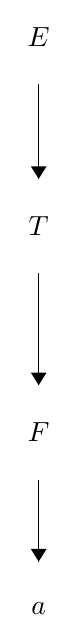
\begin{tikzpicture}[scale=0.2]
	\tikzstyle{every node}+=[inner sep=0pt]
	\draw (31.3,-11.1) node {$E$};
	\draw (31.3,-23.1) node {$T$};
	\draw (31.3,-47.4) node {$a$};
	\draw (31.3,-36.2) node {$F$};
	\draw [black] (31.3,-14.1) -- (31.3,-20.1);
	\fill [black] (31.3,-20.1) -- (31.8,-19.3) -- (30.8,-19.3);
	\draw [black] (31.3,-26.1) -- (31.3,-33.2);
	\fill [black] (31.3,-33.2) -- (31.8,-32.4) -- (30.8,-32.4);
	\draw [black] (31.3,-39.2) -- (31.3,-44.4);
	\fill [black] (31.3,-44.4) -- (31.8,-43.6) -- (30.8,-43.6);
	\end{tikzpicture}
\end{center}

Derivation for $a$: $E \rightarrow T \rightarrow F \rightarrow a$ \\

\noindent
b. \\
Parse tree for $a + a$: \\
\begin{center}
	\begin{tikzpicture}[scale=0.2]
	\tikzstyle{every node}+=[inner sep=0pt]
	\draw (42.4,-7.5) node {$E$};
	\draw (31.3,-18.5) node {$E$};
	\draw (31.3,-41) node {$F$};
	\draw (31.3,-29.2) node {$T$};
	\draw (31.3,-53.4) node {$a$};
	\draw (43.2,-53.4) node {$+$};
	\draw (52.9,-53.4) node {$a$};
	\draw (52.9,-18.5) node {$T$};
	\draw (52.9,-29.2) node {$F$};
	\draw [black] (40.27,-9.61) -- (33.43,-16.39);
	\fill [black] (33.43,-16.39) -- (34.35,-16.18) -- (33.65,-15.47);
	\draw [black] (31.3,-21.5) -- (31.3,-26.2);
	\fill [black] (31.3,-26.2) -- (31.8,-25.4) -- (30.8,-25.4);
	\draw [black] (31.3,-32.2) -- (31.3,-38);
	\fill [black] (31.3,-38) -- (31.8,-37.2) -- (30.8,-37.2);
	\draw [black] (31.3,-44) -- (31.3,-50.4);
	\fill [black] (31.3,-50.4) -- (31.8,-49.6) -- (30.8,-49.6);
	\draw [black] (42.45,-10.5) -- (43.15,-50.4);
	\fill [black] (43.15,-50.4) -- (43.63,-49.59) -- (42.63,-49.61);
	\draw [black] (44.47,-9.67) -- (50.83,-16.33);
	\fill [black] (50.83,-16.33) -- (50.64,-15.41) -- (49.91,-16.1);
	\draw [black] (52.9,-21.5) -- (52.9,-26.2);
	\fill [black] (52.9,-26.2) -- (53.4,-25.4) -- (52.4,-25.4);
	\draw [black] (52.9,-32.2) -- (52.9,-50.4);
	\fill [black] (52.9,-50.4) -- (53.4,-49.6) -- (52.4,-49.6);
	\end{tikzpicture}
\end{center}

\noindent
Derivation for $a + a$: $E \rightarrow E + T \rightarrow T + T \rightarrow T + F \rightarrow F + a \rightarrow a + a$ \\

\noindent
c. \\
Parse tree for $a + a + a$: \\
\begin{center}
	\begin{tikzpicture}[scale=0.2]
	\tikzstyle{every node}+=[inner sep=0pt]
	\draw (42.4,-7.5) node {$E$};
	\draw (15.4,-22.9) node {$E$};
	\draw (15.4,-42.7) node {$F$};
	\draw (15.4,-32.7) node {$T$};
	\draw (15.4,-52.4) node {$a$};
	\draw (43.3,-52.4) node {$+$};
	\draw (52.9,-52.4) node {$a$};
	\draw (52.9,-18.5) node {$T$};
	\draw (52.9,-32.7) node {$F$};
	\draw (24.2,-11.6) node {$E$};
	\draw (32.3,-22.9) node {$T$};
	\draw (32.3,-52.4) node {$a$};
	\draw (24.2,-52.4) node {$+$};
	\draw [black] (15.4,-25.9) -- (15.4,-29.7);
	\fill [black] (15.4,-29.7) -- (15.9,-28.9) -- (14.9,-28.9);
	\draw [black] (15.4,-35.7) -- (15.4,-39.7);
	\fill [black] (15.4,-39.7) -- (15.9,-38.9) -- (14.9,-38.9);
	\draw [black] (15.4,-45.7) -- (15.4,-49.4);
	\fill [black] (15.4,-49.4) -- (15.9,-48.6) -- (14.9,-48.6);
	\draw [black] (42.46,-10.5) -- (43.24,-49.4);
	\fill [black] (43.24,-49.4) -- (43.72,-48.59) -- (42.72,-48.61);
	\draw [black] (44.47,-9.67) -- (50.83,-16.33);
	\fill [black] (50.83,-16.33) -- (50.64,-15.41) -- (49.91,-16.1);
	\draw [black] (52.9,-21.5) -- (52.9,-29.7);
	\fill [black] (52.9,-29.7) -- (53.4,-28.9) -- (52.4,-28.9);
	\draw [black] (52.9,-35.7) -- (52.9,-49.4);
	\fill [black] (52.9,-49.4) -- (53.4,-48.6) -- (52.4,-48.6);
	\draw [black] (26.504,-9.684) arc (124.87897:80.51176:17.638);
	\fill [black] (26.5,-9.68) -- (27.45,-9.64) -- (26.87,-8.82);
	\draw [black] (22.36,-13.97) -- (17.24,-20.53);
	\fill [black] (17.24,-20.53) -- (18.13,-20.21) -- (17.34,-19.59);
	\draw [black] (25.95,-14.04) -- (30.55,-20.46);
	\fill [black] (30.55,-20.46) -- (30.49,-19.52) -- (29.68,-20.1);
	\draw [black] (24.2,-14.6) -- (24.2,-49.4);
	\fill [black] (24.2,-49.4) -- (24.7,-48.6) -- (23.7,-48.6);
	\draw [black] (32.3,-25.9) -- (32.3,-49.4);
	\fill [black] (32.3,-49.4) -- (32.8,-48.6) -- (31.8,-48.6);
	\end{tikzpicture}
\end{center}

\noindent
Derivation for $a + a + a$: $E \rightarrow E + T \rightarrow T + T + T \rightarrow F + T + F \rightarrow$ \\
$F + F + T \rightarrow F + F + F \rightarrow a + F + F \rightarrow a + a + F \rightarrow a + a + a$ \\

\noindent
d. \\
\noindent
Parse tree for $((a))$: \\
\begin{center}
	\begin{forest}
		[E [T [F [(E) [(T) [(F) [((E)) [((T)) [((F)) [a]]]]]]]]]]]
	\end{forest}
\end{center}

\noindent
Derivation for $((a))$:  $E \rightarrow T \rightarrow F \rightarrow (E) \rightarrow (T) \rightarrow (F) \rightarrow ((E)) $  \\
$ \rightarrow ((T)) \rightarrow ((F)) \rightarrow ((a)) $ \\

%*********************************************************************************
% 2.4 b, c, e, f here

\noindent
2.4 \\
Give context-free grammars that generate the following languages. \\
In all parts, the alphabet $\sum$ is $\{0,1\}$. \\

\noindent
b. \{w| w starts and ends with the same symbol\} \\
$ S \rightarrow 0P0|1P1| \epsilon $ \\
$ P \rightarrow 0P|1P| \epsilon $ \\

\noindent
c. \{w| the length of w is odd\} \\
$ S \rightarrow 0|1|00S|01S|10S|11S $ \\

\noindent
e. \{w| w = $w\textsuperscript{R}$, that is, w is a palindrome\} \\
$ S \rightarrow 0|1|0S0|1S1| \epsilon $ \\

\noindent
f. The empty set \\
$ S \rightarrow \epsilon $ \\

%*********************************************************************************
% 2.5 here

\noindent
2.5 \\
Give informal descriptions and state diagrams of pushdown automata for \\
the languages in Exercise 2.4. \\

\noindent
a. \{w| w contains at least three 1s\}\\

\noindent
Informal: In this grammar, there is no need of a stack (as seen in the diagram). In the grammar only the input is read, and the input is only accepted when there is at least three 1's. The only time the machine will accept a string in this case is when at least three 1's are present; otherwise it is rejected. \\\\
\noindent
Pushdown Automata:\\
\begin{center}
	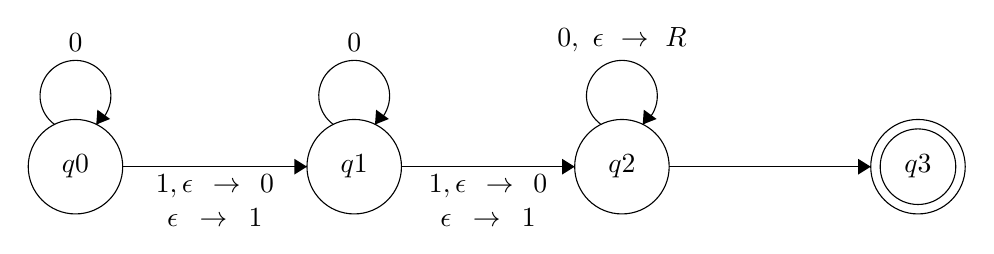
\begin{tikzpicture}[scale=0.2]
	\tikzstyle{every node}+=[inner sep=0pt]
	\draw [black] (12.4,-29.9) circle (3);
	\draw (12.4,-29.9) node {$q0$};
	\draw [black] (30.1,-29.9) circle (3);
	\draw (30.1,-29.9) node {$q1$};
	\draw [black] (47.1,-29.9) circle (3);
	\draw (47.1,-29.9) node {$q2$};
	\draw [black] (65.9,-29.9) circle (3);
	\draw (65.9,-29.9) node {$q3$};
	\draw [black] (65.9,-29.9) circle (2.4);
	\draw [black] (15.4,-29.9) -- (27.1,-29.9);
	\fill [black] (27.1,-29.9) -- (26.3,-29.4) -- (26.3,-30.4);
	\draw (21.25,-30.4) node [below] [text width=2cm,align=center] {$1,\epsilon\mbox{ }\rightarrow\mbox{ }0$\\$\epsilon\mbox{ } \rightarrow\mbox{ }1$};
	\draw [black] (33.1,-29.9) -- (44.1,-29.9);
	\fill [black] (44.1,-29.9) -- (43.3,-29.4) -- (43.3,-30.4);
	\draw (38.6,-30.4) node [below] [text width=2cm,align=center] {$1,\epsilon\mbox{ }\rightarrow\mbox{ }0$\\$\epsilon\mbox{ } \rightarrow\mbox{ } 1$};
	\draw [black] (50.1,-29.9) -- (62.9,-29.9);
	\fill [black] (62.9,-29.9) -- (62.1,-29.4) -- (62.1,-30.4);
	\draw [black] (11.077,-27.22) arc (234:-54:2.25);
	\draw (12.4,-22.65) node [above] {$0$};
	\fill [black] (13.72,-27.22) -- (14.6,-26.87) -- (13.79,-26.28);
	\draw [black] (28.777,-27.22) arc (234:-54:2.25);
	\draw (30.1,-22.65) node [above] {$0$};
	\fill [black] (31.42,-27.22) -- (32.3,-26.87) -- (31.49,-26.28);
	\draw [black] (45.777,-27.22) arc (234:-54:2.25);
	\draw (47.1,-22.65) node [above] {$0,\mbox{ }\epsilon\mbox{ }\rightarrow\mbox{ }R$};
	\fill [black] (48.42,-27.22) -- (49.3,-26.87) -- (48.49,-26.28);
	\end{tikzpicture}
\end{center}

\noindent
b. \{w| w starts and ends with the same symbol\} \\
\noindent
Informal: In this grammar, there is an assumption that there is only one symbol in the string
that can be accepted without the use of a stack. If there is more than one symbol in the string,
then all of the symbols are put into the stack in order. We also check to see whether the last
symbol is the one being read. If it is, and this symbol matches with the symbol on the stack,
and if all the input has been checked with no input left, then we accept that state. Otherwise
we reject the input.

\noindent
Pushdown Automata:\\
\begin{center}
	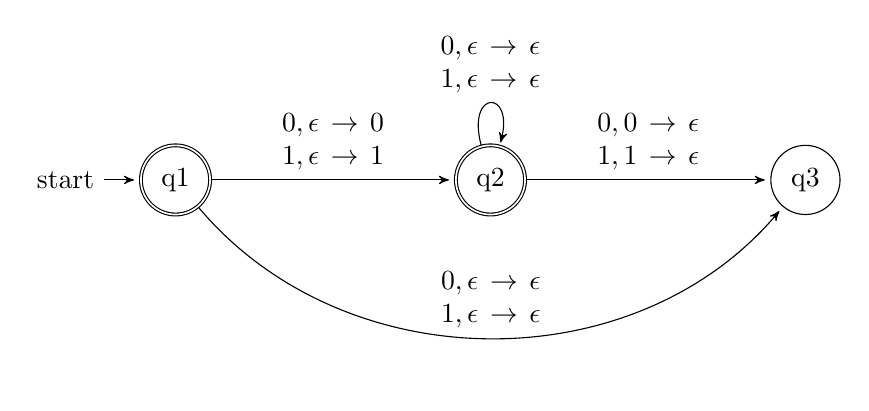
\begin{tikzpicture}[>=stealth',shorten >=2pt, auto, node distance=4cm]
	% Nodes {q1, q2, q3, q4, q5, etc}
	\node [state, initial, accepting] 		(q1) 				 {q1};
	\node [state, accepting] 				(q2)  [right of=q1]  {q2};
	\node [state]   	                    (q3)  [right of=q2]  {q3};
	
	% Paths
	\path [->] 	(q1) edge 	node	[text width=2cm,align=center] 
	{$0, \epsilon \rightarrow 0$ \\ $1, \epsilon \rightarrow 1$}	(q2);
	
	\path [->] 	(q2) edge 	node	[text width=2cm,align=center] 
	{$0, 0 \rightarrow \epsilon$ \\ $1, 1 \rightarrow \epsilon$}	(q3);
	
	\path [->] 	(q2) edge [loop above] 	node	[text width=2cm,align=center] 
	{$0, \epsilon \rightarrow \epsilon$ \\ $1, \epsilon \rightarrow \epsilon$}		(q2);
	
	\path [->] 	(q1) edge [bend right=50] node [text width=2cm,align=center]	
	{$0, \epsilon \rightarrow \epsilon$ \\ $1, \epsilon \rightarrow \epsilon$}	(q3);
	
	\end{tikzpicture} \\
\end{center}

\noindent
c. \{w| the length of w is odd\} \\
\noindent
Informal: In this grammar, there is no need of a stack. In this grammar, we only read
the input and this input is also only accepted when there is an odd length.

\noindent
Pushdown Automata:\\
\begin{center}
	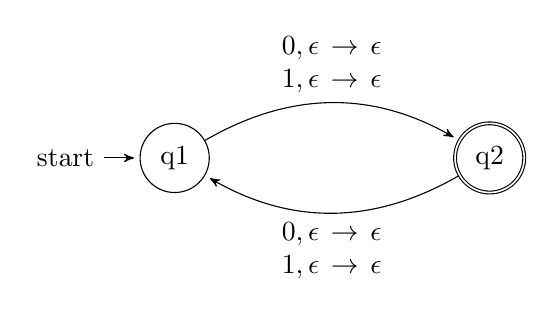
\begin{tikzpicture}[>=stealth',shorten >=2pt, auto, node distance=4cm]
	% Nodes {q1, q2, q3, q4, q5, etc}
	\node [state, initial] 			(q1) 				 {q1};
	\node [state, accepting]        (q2)  [right of=q1]  {q2};
	
	% Paths
	\path [->] 	(q1) edge [bend left]   node	[text width=2cm,align=center]	
	{$0, \epsilon \rightarrow \epsilon$ \\ $1, \epsilon \rightarrow \epsilon$}		(q2);
	
	\path [->] 	(q2) edge [bend left] 	node	[text width=2cm,align=center]	
	{$0, \epsilon \rightarrow \epsilon$ \\ $1, \epsilon \rightarrow \epsilon$}		(q1);
	
	\end{tikzpicture}
\end{center}

\noindent
d. \{w| the length of w is odd and its middle symbol is a 0\}\\
\noindent
Informal: In this grammar, the input is read by the pushdown automata and each symbol is
placed onto the stack. At each point, the pushdown automata guesses if the input in the middle
or if the next symbol read is in the middle of the string. If the next symbol read is the middle
of the string then it does not get read onto the stack. After this, we pop symbols off the stack
if they match the input symbols that were read. If the symbols that are popped match the symbols
that were pushed earlier, and the stack is empty as the input is finished, we accept the state.
Otherwise we reject the state.


\noindent
Pushdown Automata:\\
\begin{center}
	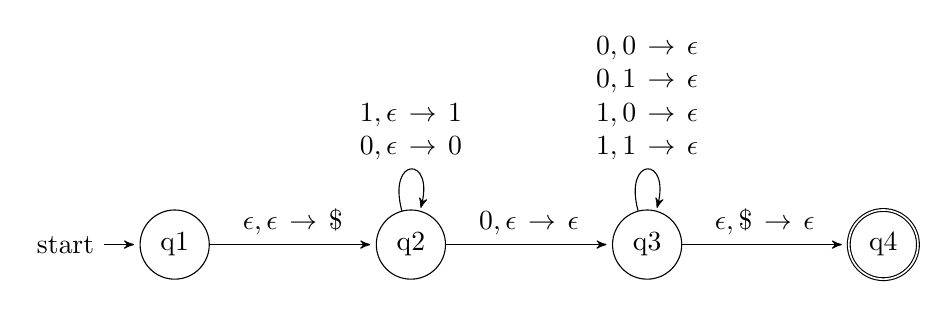
\begin{tikzpicture}[>=stealth',shorten >=2pt, auto, node distance=3cm]
	% Nodes {q1, q2, q3, q4, q5, etc}
	\node [state, initial] 		(q1) 				 {q1};
	\node [state] 				(q2)  [right of=q1]  {q2};
	\node [state]    			(q3)  [right of=q2]  {q3};
	\node [state, accepting]	(q4)  [right of=q3]  {q4};
	
	% Paths
	\path [->] 	(q1) edge 				node	[text width=2cm,align=center]	
	{$\epsilon, \epsilon \rightarrow \$$}	(q2);
	
	\path [->] 	(q2) edge 				node	[text width=2cm,align=center]	
	{$0, \epsilon \rightarrow \epsilon$}	(q3);
	
	\path [->] 	(q2) edge [loop above] 	node	[text width=2cm,align=center]	
	{$1, \epsilon \rightarrow 1$ \\ $0, \epsilon \rightarrow 0$}		(q2);
	
	\path [->] 	(q3) edge 				node	[text width=2cm,align=center]	
	{$\epsilon, \$ \rightarrow \epsilon$}		(q4);
	
	\path [->] 	(q3) edge [loop above] 	node	[text width=2cm,align=center]	
	{$0, 0 \rightarrow \epsilon$ \\ $0, 1 \rightarrow \epsilon$ \\ $1, 0 \rightarrow \epsilon$ \\ $1, 1 \rightarrow \epsilon$}	(q3);
	
	\end{tikzpicture} \\
\end{center}

\noindent
e. \{w| w = $w\textsuperscript{R}$, that is, w is a palindrome\} \\
\noindent
Informal: In this grammar, the input is read by the pushdown automata and each symbol is
placed onto the stack. At each point, the pushdown automata guesses if the input in the middle
or if the next symbol read is in the middle of the string. If the next symbol read is the middle
of the string then it does not get read onto the stack. After this, we pop symbols off the stack
if they match the input symbols that were read. If the symbols that are popped match the symbols
that were pushed earlier, and the stack is empty as the input is finished, we accept the state.
Otherwise we reject the state.

\noindent
Pushdown Automata: \\
\begin{center}
	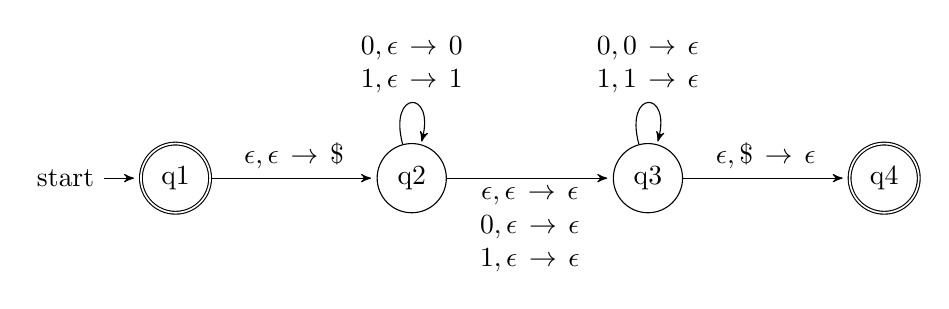
\begin{tikzpicture}[>=stealth',shorten >=2pt, auto, node distance=3cm]
	% Nodes {q1, q2, q3, q4, q5, etc}
	\node [state, initial, accepting] 		(q1) 				 {q1};
	\node [state] 				(q2)  [right of=q1]  {q2};
	\node [state]    			(q3)  [right of=q2]  {q3};
	\node [state, accepting]	(q4)  [right of=q3]  {q4};
	
	% Paths
	\path [->] 	(q1) edge 				node	[text width=2cm,align=center]	
	{$\epsilon, \epsilon \rightarrow \$$}	(q2);
	
	\path [->] 	(q2) edge 	[below]	node	[text width=2cm,align=center]	
	{$\epsilon, \epsilon \rightarrow \epsilon$ \\ $0, \epsilon \rightarrow \epsilon$ \\ $1, \epsilon \rightarrow \epsilon$}	(q3);
	
	\path [->] 	(q2) edge [loop above] 	node	[text width=2cm,align=center]	
	{$0, \epsilon \rightarrow 0$ \\ $1, \epsilon \rightarrow 1$}		(q2);
	
	\path [->] 	(q3) edge 				node	[text width=2cm,align=center]	
	{$\epsilon, \$ \rightarrow \epsilon$}		(q4);
	
	\path [->] 	(q3) edge [loop above] 	node	[text width=2cm,align=center]	
	{$0, 0 \rightarrow \epsilon$ \\ $1, 1 \rightarrow \epsilon$}	(q3);
	
	\end{tikzpicture} \\
\end{center}

\noindent
f. The empty set \\
\noindent
Informal: In this grammar, the language only accepts an empty set so it implies that
it does not terminate any derivation. And if none of the derivations are terminated,
that means that no string is accepted by the CFG, including the empty string.

\noindent
Pushdown Automata:\\
\begin{center}
	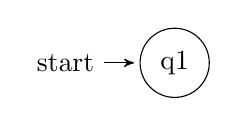
\begin{tikzpicture}[>=stealth',shorten >=2pt, auto, node distance=2cm]
	% Nodes {q1, q2, q3, q4, q5, etc}
	\node [state, initial] 		(q1) 				{q1};
	
	\end{tikzpicture}
\end{center}

%*********************************************************************************
% 2.6 here
\noindent
2.6 \\

\noindent
b. \\

\noindent
d. \\

%*********************************************************************************
% 2.10 here
\noindent
2.10 \\

%*********************************************************************************
% 2.11 here
\noindent
2.11 \\

%*********************************************************************************
% 2.12 here
\noindent
2.12 \\

%*********************************************************************************
% 2.13 here
\noindent
2.13 \\

%*********************************************************************************
% 2.14 here
\noindent
2.14 \\

%*********************************************************************************
% 2.26 here
\noindent
2.26 \\

%*********************************************************************************
% 2.30 here
\noindent
2.30 \\

%*********************************************************************************
% 2.31 here
\noindent
2.31 \\

%*********************************************************************************
% 2.32 here
\noindent
2.32 \\

%*********************************************************************************
% 2.47 here
\noindent
2.47 \\

\end{document}
